\scanpage{6}
\deleted{\unsure{$G$-$\underline F_p(G)$-Modules}} Modules de représentations de $G$ sur $\underline F_p$. Alors les termes $(\operatorname{Coker}u_2)_{\mathrm{SS}}$ et $(\operatorname{Ker}u_2)_{\mathrm{SS}}$ peuvent s'interpréter aussi comme les duals de $(\operatorname{Ker}u''_2)_{\mathrm{SS}}$ et de $(\operatorname{Coker}u''_2)_{\mathrm{SS}}$, $u''_2$ défini dans (8.3.2). Enfin \deleted{\unsure{$(\operatorname{Ker}u_1)_{\mathrm{SS}}$}} $(\operatorname{Coker}u_1)_{\mathrm{SS}}$ et $(\operatorname{Ker}u_1)_{\mathrm{SS}}$ ont aussi une interprétation simple, grâce au

\margin{\figure{\begin{tikzpicture}\draw[gray] (0,0)--(0,2.6);\end{tikzpicture}}}
\uline{Lemme} 8.4.\unsure{3}. Soit $X$ un schéma propre sur un corps $k$, de car. $p>0$. Alors pour tout $i\in\underline Z$, l'homomorphisme d'augmentation \deleted{\unsure{H}}
\[
H^i_{\mathrm{DR}}(X)\longrightarrow H^i(X,\underline O_X)
\]
induit un isomorphisme sur les parties semi-simples (pour l'opération $p$-linéaire de Frobenius).

Ceci résulte aussitôt de la suite spectrale de Hodge
\[
E_1^{a,b}=H^b(X,\underline\Omega^a_{X/k})\Longrightarrow H^\bullet_{\mathrm{DR}}(X),
\]
compte tenu que Frob opère \deleted{semi} $p$-linéairement sur cette suite spectrale \inserted{et} qu'il est nul sur $E_1^{a,b}$ pour $a\ne0$. Alors les $(E_1^{0,b})_{\mathrm{SS}}\unsure{\simeq}\ =H^b(X,\underline O_X)_{\mathrm{SS}}$ sont des cycles universels pour les $d_r$, et on gagne \ldots
\margin{Cor 8.4.\uline{\unsure{4}} (\unsure{utilis.}$\to$8.1?) les résultats de la feuille jointe (marquée 8.4.4).}
\margin{\figure{\begin{tikzpicture}[x=1cm,y=1cm]
\draw (0,3.6) .. controls (.2,3.6) and (.15,3.1) .. (.15,2.2) .. controls (.15,1.9) and (.5,1.8) .. (.8,1.7) .. controls (.4,1.6) and (.3,1.3) .. (.15,.2);
\end{tikzpicture}}}

Mettant ensemble les renseignements obtenus, \deleted{et en même temps, pour des raisons de commodité, transformant par dualité de Poincaré l'\unsure{homomorphisme} $u''_2$ de (8.3.2), de sorte qu'on trouve
\[
(8.4.2)\qquad u_2\text{ est can. isomorphe à}
\]}
\margin{\uline{(oubli dans 8.3!)}}
on trouve:

\margin{\figure{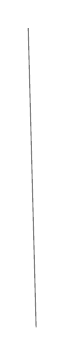
\begin{tikzpicture}\draw[gray] (0,0)--(-.1,3.8);\end{tikzpicture}}}
``\uline{Théorème}'' 8.5. En admettant lesingrédients précédents pour la cohomologie cristalline (\inserted{formule des} coefficients universels, dualité de Poincaré, théorème \unsure{de} Lefschetz \inserted{``faible''}\deleted{y compris pour les groupes de torsion}\inserted{sans négliger la torsion}), on obtient une suite exacte, relative à une variété lisse projective connexe $X\subset P_k^r$ \inserted{de dimension $n$} sur un corps parfait de car. $p>0$, et une section hyperplane (ou par une hypersurface, \inserted{de degré $d\geq1$} cela s'y ramène \ldots) $Y$ lisse de dimension $n-1$:
\deleted{\diagram{\unsure{$(8.5.1)$\quad\begin{tikzcd}[ampersand replacement=\&,column sep=small]
0\arrow[r]\&(\operatorname{Ker}v)\arrow[r]\&(\operatorname{Coker}v)
\end{tikzcd}}}
\[
(E(Y)\otimes_W k)_{\mathrm{SS}}\qquad\operatorname{Coker}v_{\mathrm{DR}}
\]}

\mspage{5}
